%%%%%%%%%%%%%%%%%%%%%%%%%%%%%%%%%%%%%%%%%%%%%%%%%%%%%%%%%%%%%%%%%%%%%
% LaTeX Template: Project Titlepage Modified (v 0.1) by rcx
%
% Original Source: http://www.howtotex.com
% Date: February 2014
% 
% This is a title page template which be used for articles & reports.
% 
% This is the modified version of the original Latex template from
% aforementioned website.
% 
%%%%%%%%%%%%%%%%%%%%%%%%%%%%%%%%%%%%%%%%%%%%%%%%%%%%%%%%%%%%%%%%%%%%%%

\documentclass[12pt]{article}
\usepackage[a4paper]{geometry}
\usepackage[myheadings]{fullpage}
\usepackage{fancyhdr}
\usepackage{lastpage}
\usepackage{graphicx, wrapfig, subcaption, setspace, booktabs}
\usepackage[T1]{fontenc}
\usepackage[font=small, labelfont=bf]{caption}
\usepackage{fourier}
\usepackage[protrusion=true, expansion=true]{microtype}
\usepackage[english]{babel}
\usepackage{sectsty}
\usepackage{url, lipsum}
\usepackage{tabularx}

\newcommand\boldblue[1]{\textcolor{blue}{\textbf{#1}}}
\newcommand{\HRule}[1]{\rule{\linewidth}{#1}}
\onehalfspacing
\setcounter{tocdepth}{5}
\setcounter{secnumdepth}{5}

%-------------------------------------------------------------------------------
% HEADER & FOOTER
%-------------------------------------------------------------------------------
\pagestyle{fancy}
\fancyhf{}
\setlength\headheight{15pt}
\fancyhead[L]{CHARM}
\fancyhead[R]{Carleton University}
\fancyfoot[R]{Page \thepage\ of \pageref{LastPage}}
%-------------------------------------------------------------------------------
% TITLE PAGE
%-------------------------------------------------------------------------------

\begin{document}
\bibliographystyle{ieeetr}

\title{ \normalsize \textsc{}
		\\ [2.0cm]
		\HRule{0.5pt} \\
		\LARGE \textbf{{Carleton High Altitude Radiometer}}\\
		\large \textbf{{Project Proposal}}\\
		\large \textbf{{Canadian Stratospheric Balloon Experiment Design Challenge}}
		\HRule{2pt} \\ [0.5cm]
		\normalsize \today \vspace*{2\baselineskip}\\
		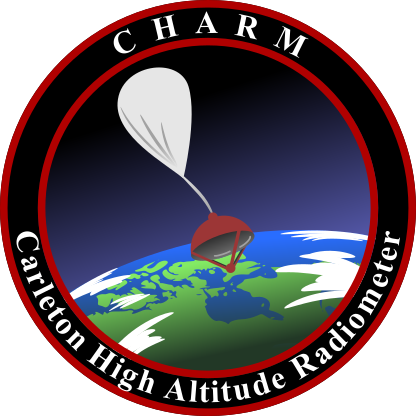
\includegraphics[scale=0.6]{Figures/CHARM.png}	\vspace*{2\baselineskip} \\
		\textsc{
		David Bascelli \quad Team Lead \\
		Jacob Booth \quad Sensor Lead \\
		}}
		
\date{}
	
\author{
		Carleton University \\
		}
	


\maketitle

\newpage

\tableofcontents
\newpage

\listoffigures
\newpage

\listoftables
\newpage

%-------------------------------------------------------------------------------
% Section title formatting
\sectionfont{\scshape}
%-------------------------------------------------------------------------------

%-------------------------------------------------------------------------------
% BODY
%-------------------------------------------------------------------------------

\section{Executive Summary}
Microwave remote sensing has been a common payload on earth observation satellites since the early days of space-flight. In as early as 1962, a radiometer on-board the Mariner 2 mission measured the surface temperature of Venus. 1968 Saw the first space-born earth observation radiometer on-board the  Cosmos 243 satellite, which measured atmospheric water vapour and global ice cover. Many different radiometer configurations can make a wide array of different geological, biological, and climate measurements. The CHARM project will design and manufacture a C-band balloon mounted microwave radiometer for the purpose of measuring soil moisture content over a large area. Soil moisture measurements are crucial in predicting local weather conditions and monitoring climate change. Incorporating soil moisture measurements into weather and climate models allows for more accurate medium term weather forecasts and can also give clues about future droughts, crop yields, and water resource management. Currently, most radiometric data comes from space-born radiometers, such as those on the SMAP or SMOS satellites. To achieve high resolution and accuracy, these space-born radiometers utilize cryogenic components, complex phased array or synthetic aperture technologies, and require large and very directional antennas. Our belief is that measurements of similar similar quality could be performed from a high altitude balloon at significantly reduced cost. 

\newpage

\section{Proposal}
\subsection{Scientific Objectives}

Our scientific objective is to make low cost measurements of soil moisture content using a balloon born microwave radiometer. The payload will take wide-band measurements of the noise equivalent temperature of the ground and determine soil moisture content through a modification of the zeroth order radiative transfer model (ZRT Model). A basic dielectric model will be used to solve for volumetric moisture content. \cite{ulaby_fung_moore_1986} A NADIR pointing antenna will extend from the pelican case to take measurements of the background microwave emissions coming from the ground. The radiometer will be of the Dicke type, which compares measurements to a known noise source to eliminate the effect of varying gain due to extreme temperatures. A 9-axis inertial measurement unit (IMU) will measure linear acceleration, angular rates, and magnetic field strength to determine the attitude of the payload. GPS data will be saved to track the location of the payload as it passes over the earth. With the attitude and GPS data, a map of soil moisture content under the payloads flight path will be able to be made. 

A Balloon born microwave radiometer to measure soil moisture was selected for several reasons. First, soil moisture content was chosen to be measured because of its importance to weather and climate monitoring.\cite{Pan2001} Soil moisture measurements are useful in many different circumstances. Climate models, weather predictions, crop yield estimation and water resource management systems all benifit from accurate and up to date measurements of ground moisture content. Soil moisture measurements have also proved useful in predicting wildfires.\cite{chaparro_piles_vall-llossera_2016,krueger_ochsner_quiring_engle_carlson_twidwell_fuhlendorf_2017} Second, measuring soil moisture content from radiometers is reasonably common and a significant amount of literature exists on the topic. Most literature either concerns satellite born radiometers, aircraft born radiometers, or static ground based radiometers. \cite{Hanington,Kerr2001,ulaby_fung_moore_1986,Friesen2008,Schmugge1994} By exploring the possibility of balloon based radiometers and by attempting more advanced soil moisture estimation techniques, we can achieve a degree of novelty while still having a wealth of proven literature and designs to aid us. Third, balloon mounted radiometers have several advantages to static, aircraft mounted, and satellite radiometers. Due to the balloon's proximity to the ground compared to low earth orbit, balloon born radiometers can achieve greater resolution with smaller and less directional antennas. Balloon radiometers can achieve much greater loiter times than aircraft born radiometers, although balloons are uncontrolled. Balloon born radiometers also have the advantage of being significantly cheaper to operate than aircraft or satellite mounted radiometers. A trade study was performed in table \ref{tab:algorithm_parameters}, and it can be seen that balloon born radiometers offer a unique performance compromise at very low cost when compared to aircraft mounted or satellite based radiometers.

\begin{table}[!h]
	\centering
	\vspace{0.5cm}
	\renewcommand{\arraystretch}{1.3}
	\caption{Radiometer Vehicle Trade Study. }
	\label{tab:algorithm_parameters}
	\begin{tabularx}{\textwidth}{llll}
		\toprule
						& Satellite & Aircraft & Balloon \\		
		\midrule
		Cost			&\$\$\$&\$\$&\$ \\ 
		Antenna Size 			&Large&Small&Small/Medium \\
		Resolution 				&Low Resolution&High Resolution&Medium Resolution \\ 
		Atmospheric Effects		&High&Low&Moderate \\ 
		Loiter Time				&N/A&Up to 6 hours&6 - 48 Hours \\ 
		Controllability			&Uncontrolled but predictable&Controlled&Uncontrolled 
	\end{tabularx}
\end{table}

Lastly, soil moisture retrieval from radiometric data is one of the simpler radiometer configurations to design and operate, allowing our team to gain experience with radiometer principals before attempting more advanced designs. Thus, a microwave radiometer was chosen as our balloon payload because of its many geoscientific applications, the wealth of literature and design aids, their suitability to the high altitude balloon environment, and because it allows us to gain experience with a relatively simple radiometer configuration.

 
\subsection{Experiment Design}
The antenna will either be terminated with a coaxial cable at the antenna, or wave-guides will be used to guide C-band microwaves into the pelican case to keep all connections within the pelican case.
\subsubsection{Radiometer Block Diagram}
David
\subsubsection{Attitude Determination}
Jacob
\subsubsection{Experimental Procedures}
David
\subsubsection{Resources}
David
\subsubsection{Technical Risk Assessment}
Jacob
\begin{enumerate}
\item Human
\cite{omar_el-kassaby_abdelghaffar_2017}
\item Technical and Environmental
\end{enumerate}
\subsection{Management}
David
\subsubsection{Team Structure}
\subsubsection{Project Time-line}
\subsubsection{Budget}
\subsubsection{Managerial Risk Assessment}

\subsection{Outreach}
Jacob
\subsubsection{Public Outreach}
\subsubsection{Academic Outreach}

\section{Conclusion}

%-------------------------------------------------------------------------------
% REFERENCES
%-------------------------------------------------------------------------------
\newpage
\section{References}

\bibliography{radiometer}

\section{Appendix}


\end{document}
